\subsection{Algoritmen voor scheduling}

\subsubsection{Criteria bij scheduling voor korte termijn}

Hoofddoel is het toewijzen van processortijd dat een of meer aspecten van het systeemgedrag worden geoptimaliseerd.

Een aantal criteria worden vaak opgesteld waarmee verschillende schedulingstrategieën kunnen worden beoordeeld.

\textbf{Gebruiker tegenover systeem}

We kunnen een onderscheid maken tussen gebruikersgerichte criteria en 
systeemgerichte cirteria. 
Gebruikersgerichte criteria: antwoordtijd (tijd tussen de aanvraag en de output).

Systeemgerichte criteria: Effectief en efficiënt gebruik van de processor.

\textbf{Prestaties}

We kunnen een onderscheid maken tussen prestatiegerichte criteria en die dat niet prestatiegericht zijn. 

Prestatiegericht: Deze zijn quantitatief, makkelijk te meten. (bv. Antwoordtijd en de doorvoer).

Niet-prestatie gericht: Deze zijn kwalitatie, deze zijn moeilijk te meten. (bv. Voorspelbaarheid)

\begin{landscape}

%The first thing you need to do is add \usepackage{multirow} to the preamble[3]. This then provides the command needed for spanning rows: \multirow{''num_rows''}{''width''}{''contents''}. The arguments are pretty simple to deduce (* for the width means the content's natural width).

\begin{table}
\def\arraystretch{1.5}%  1 is the default, change whatever you need
\centering     % optional, probably makes it look better to have it centered on the page
\begin{tabular}{ |l| p{19cm} | }
\hline
\multicolumn{2}{ |c| }{Gebruikersgericht, samenhangend met prestaties} \\
\hline
Omlooptijd & Dit is het tijdsinterval tussen het indienen en het voltooien van een proces.
Hiertoe behoren de werkelijke uitvoeringstijd en de tijd die wordt besteed aan het wachten op systeembronnen, waaronder de processor. Dit is een geschikte meeteenheid voor een batchtaak. \\ \hline
Antwoordtijd & Bij een interactieve toepassing is dit de tijd tussen het indienen van een verzoek en het moment waarop de ontvangst van het antwoord begint. Vaak kan een proces beginnen met het produceren van een bepaalde uitvoer terwijl de verwerking van het verzoek wordt voortgezet. Dit is daarom vanuit gebruikersoogpunt een beter meeteenheid dan de omlooptijd. Het schedulingsysteem moet proberen een kleine antwoordtijd te bereiken en het aantal interactieve gebruikers met een aanvaardbare antwoordtijd te maximaliseren. \\ \hline
Deadlines & Kunnen deadlines voor het voltooien van processon worden gespecificeerd, dan moet het schedulingsysteem andere doelen ondergeschikt maken aan het maximaliseren van het aantal deadlines dat wordt gehaald. \\ \hline
\multicolumn{2}{ |c| }{Gebruikersgericht, overige} \\
\hline
Voorspelbaarheid & Een bepaalde job moet in ongeveer dezelfde tijd en tegen ongeveer dezelfde kosten worden uitgevoerd, ongeacht de belasting van het systeem. Sterk variërende antwoord- of omlooptijden storen gebruikers. Dit kan een signaal zijn voor sterk uiteenlopende systeemwerklasten of de noodzaak het systeem af te stellen om instabiliteit te verhelpen. \\ \hline
\multicolumn{2}{ |c| }{Systeemgericht, samenhangend met prestaties} \\
\hline
Doorvoer & De schedulingstrategie moet proberen het aantal processen te maximaliseren dat per tijdseenheid wordt doorgevoerd. Dit is een meeteenheid van de hoeveelheid werk die wordt uitgevoerd. De doorvoer is duidelijk afhankelijk van de gemiddelde duur van een proces, maar wordt ook bepaald door de schedulingstrategie, die de bezettingsgraad kan beïnvloeden. \\ \hline
Processorgebruik & Dit is het percentage tijd dat de processor actief is. Bij een duur, gedeeld systeem is dit een belangrijk criterium. Bij systemen voor één gebruiker en bepaalde andere systemen, bijvoorbeeld realtimesystemen, is dit criterium minder belangrijk dan enkele andere criteria. \\ \hline
\multicolumn{2}{ |c| }{Systeemgericht, overige} \\
\hline
Eerlijkheid & Ontbreken andere richtlijnen van de gebruiker of het systeem, dan moeten alle processen het zelfde worden behandeld en mag geen enkel proces verhongeren. \\ \hline
Handhaven van prioriteiten & Worden prioriteiten toegekend aan processen, dan moet de schedulingstrategie voorrang geven aan processen met een hogere prioriteit. \\ \hline
Balans bij systeembronnen & De schedulingstrategie moet de systeembronnen bezighouden. Er moet voorrang worden gegeven aan processen die weinig gebruik maken van zwaar belaste systeembronnen. Dit criterium geldt ook voor scheduling op de middellange en de lange termijn. \\ \hline
\end{tabular}
\end{table}

\end{landscape}

\subsubsection{Gebruik van prioriteiten}

De scheduler zal altijd een proces met hogere prioriteit kiezen boven een proces met lagere prioriteit. Er zijn meerdere ready queues om elk niveau prioriteit te weergeven.

\begin{figure}[htp]
    \centering
            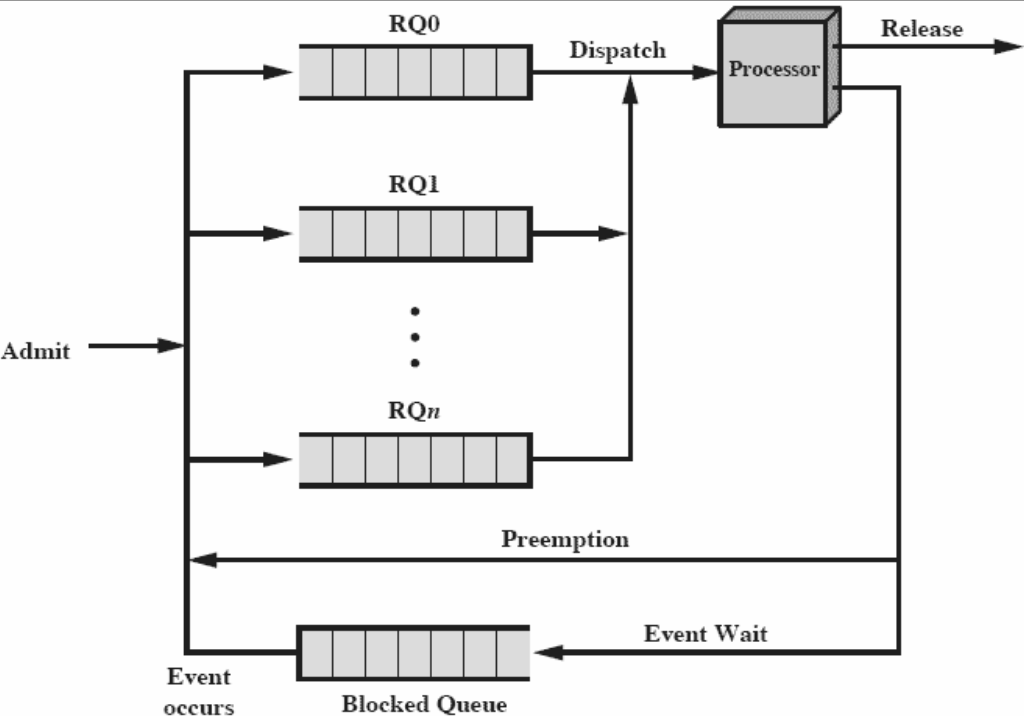
\includegraphics[width=4in]{img/gebruikvanprioriteiten.png}
        \caption{Gebruik van prioriteiten voorbeeld}
    \label{fig:Gebruik van prioriteiten voorbeeld}
\end{figure}
 
Hierboven zie hoe wachtrijen van prioriteiten in zijn werk gaan. Er wordt eerst gekeken of er een proces in RQ0 zit, zit er geen in dan gaat men kijken in RQ1, zit er dan geen in, dan kijkt men in RQ2, enz.. Hier bestaat wel kans op starvation! Als oplossing kan het proces zelf zijn prioriteit aanpassen op basis van zijn leeftijd of uitvoeringsgeschiedenis.


\subsubsection{Mogelijke strategieën voor scheduling}

Hieronder zie je de kenmerken van verschillende schedulingstrategieën

\begin{figure}[htp]
    \centering
            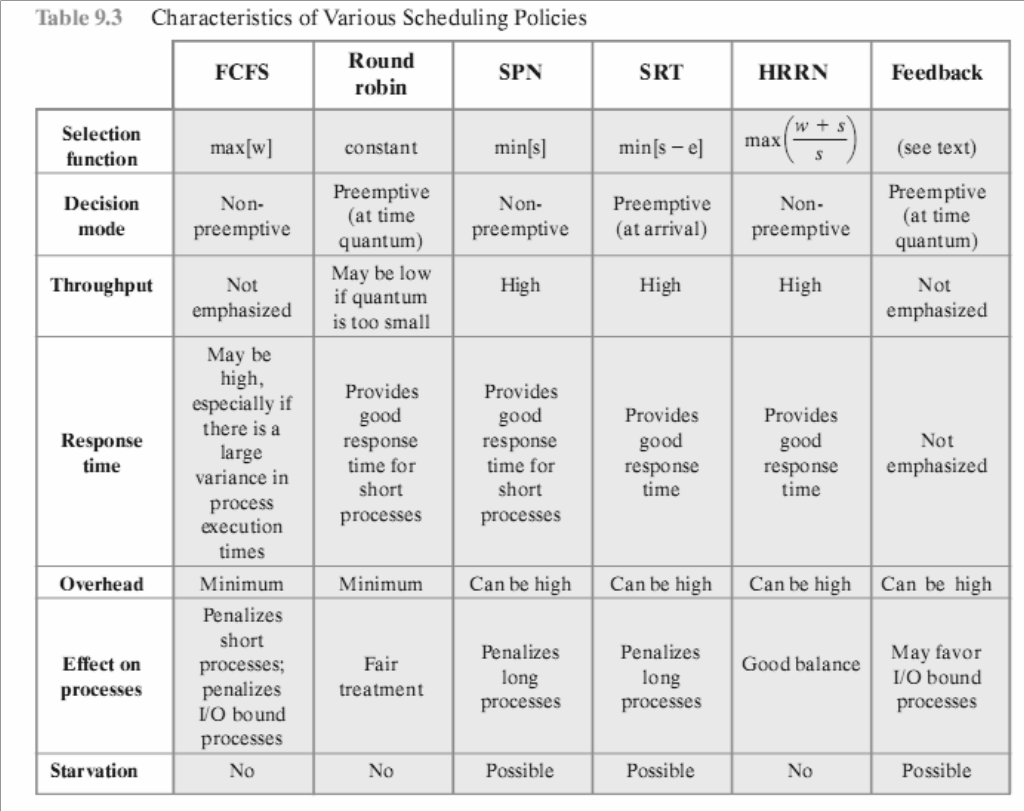
\includegraphics[width=4in]{img/schedulingpolicies.png}
        \caption{Scheduling Policies}
    \label{fig:Scheduling Policies}
\end{figure}

\textbf{De selectiefunctie} bepaald welk proces wordt geselecteerd voor uitvoering. Als het gebaseerd is op uitvoeringsgeschiedenis dan zijn de belangrijkste kwantitatieve kenmerken:
\begin{itemize}
\item W = tijd gespendeerd al wachtend
\item E = tijd gespendeerd aan uitvoering
\item S = totale bedieningstijd die vereist is voor het proces, inclusief E.
\end{itemize}

\textbf{De beslissingsmodus} bepaalt op welke tijdstippen de selectiefunctie wordt uitgevoerd. Hierin bestaan twee categorieën:
\begin{itemize}
\item Niet-preëmptief: eenmaal een proces ‘running’ is, zal het voortdoen totdat het uitgevoerd is of zichzelf blokkeert voor I/O.
\item Preëmptief: de ‘running’ toestand mag onderbroken worden en het proces mag in ‘ready’ toestand gebracht worden door het besturingssysteem. Dit kan optreden wanneer een nieuw proces wordt aangemaakt, of tijdens een interrupt of periodiek op basis van een klokinterrupt.
\end{itemize}

Voorbeeld van proces scheduling:

\begin{figure}[htp]
    \centering
            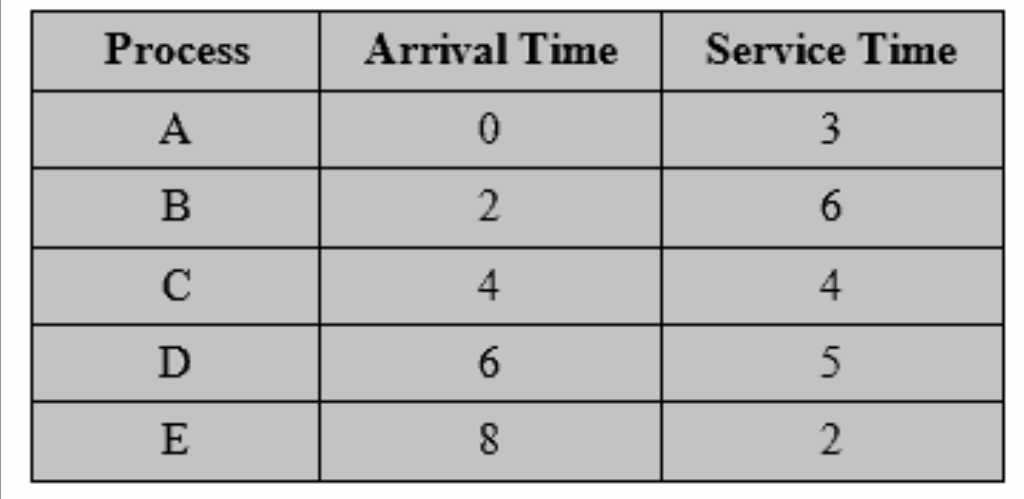
\includegraphics[width=4in]{img/processcheduling.png}
        \caption{Process Scheduling voorbeeld}
    \label{fig:Process Scheduling voorbeeld}
\end{figure}

\textbf{First come, First served}

Elk proces komt aan in de ready queue bij creatie. Wanneer het proces dat huidig wordt uitgevoerd wordt klaar is, wordt het proces dat het langste in de ready queue is geselecteerd.


\begin{figure}[htp]
    \centering
            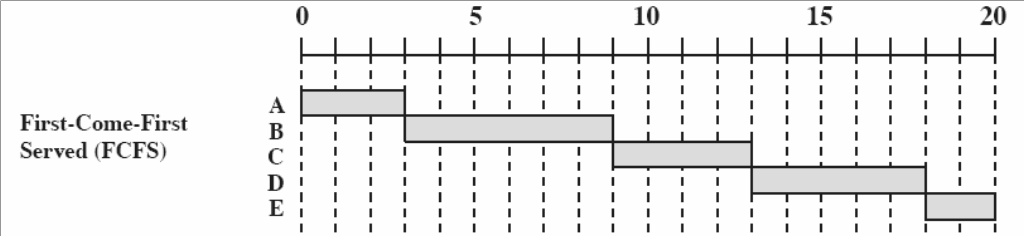
\includegraphics[width=4in]{img/firstcomefirstserved.png}
        \caption{Voorbeeld van First come, First served}
    \label{fig:First come, First served voorbeeld}
\end{figure}

Een klein proces kan wel heel lang wachten vooraleer het zijn beurt is op uitvoering. Een ander probleem is dat processorgebonden processen voorrang krijgen op I/O-gebonden processen.

\textbf{Round Robin}

Round Robin gebruikt preëmptieve onderbreking gebaseerd op een klok, dit is ook gekend als time slicing. Elk proces krijgt een slice of time (tijdsperiode) waarin hij mag uitgevoerd worden.


\begin{figure}[htp]
    \centering
            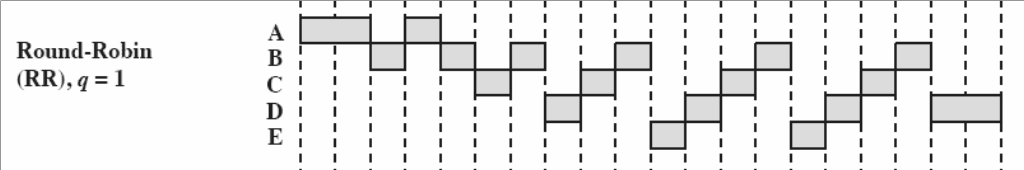
\includegraphics[width=4in]{img/roundrobin.png}
        \caption{Round Robin voorbeeld}
    \label{fig:Round Robin voorbeeld}
\end{figure}

De klokinterrupt wordt altijd met dezelfde regelmaat gegeven. Wanneer deze interrupt gebeurd wordt het ‘running’ proces in de ready queue geplaatst en wordt het eerste proces in de ready queue geselecteerd.

\textbf{Nadeel} van Round Robin is dat processen misschien tijd teveel zouden kunnen hebben. De Slice of Time kan te groot zijn voor hetgeen wat zij moeten doen. Als dit voor alle processen zo is dan komt Round Robin overeen met FCFS. Zeer korte slice of time betekent dat er veel te veel overhead zou zijn, de processor zou meer bezig zijn met het inlezen van processen uit de ready queue en processen in de ready queue plaatsen.

Bij Round Robin worden processorgebonden processen benadeeld door I/O processen omdat deze meer processortijd nodig hebben dan I/O processen en dus veel meer ‘beurten’ nodig hebben om hun taak te volbrengen.

\textbf{Virtual Round Robin} vermijdt bovenstaande oneerlijkheid. Het heeft een FCFS-wachtrij waar de I/O- processen zich in bevinden en wachten op hun I/O-gebeurtenis. Vanzodra deze optreedt worden ze in een aanvullende wachtrij geplaatst. De processen in de aanvullende wachtrij krijgen voorrang op de processen in de ready queue. Deze processen worden niet langer verwerkt dan de tijd die gelijk is aan het algemene tijdquantum min de totale tijd die besteed is aan de uitvoering van het proces sinds het uit de ready queue werd geselecteerd.



\begin{figure}[htp]
    \centering
            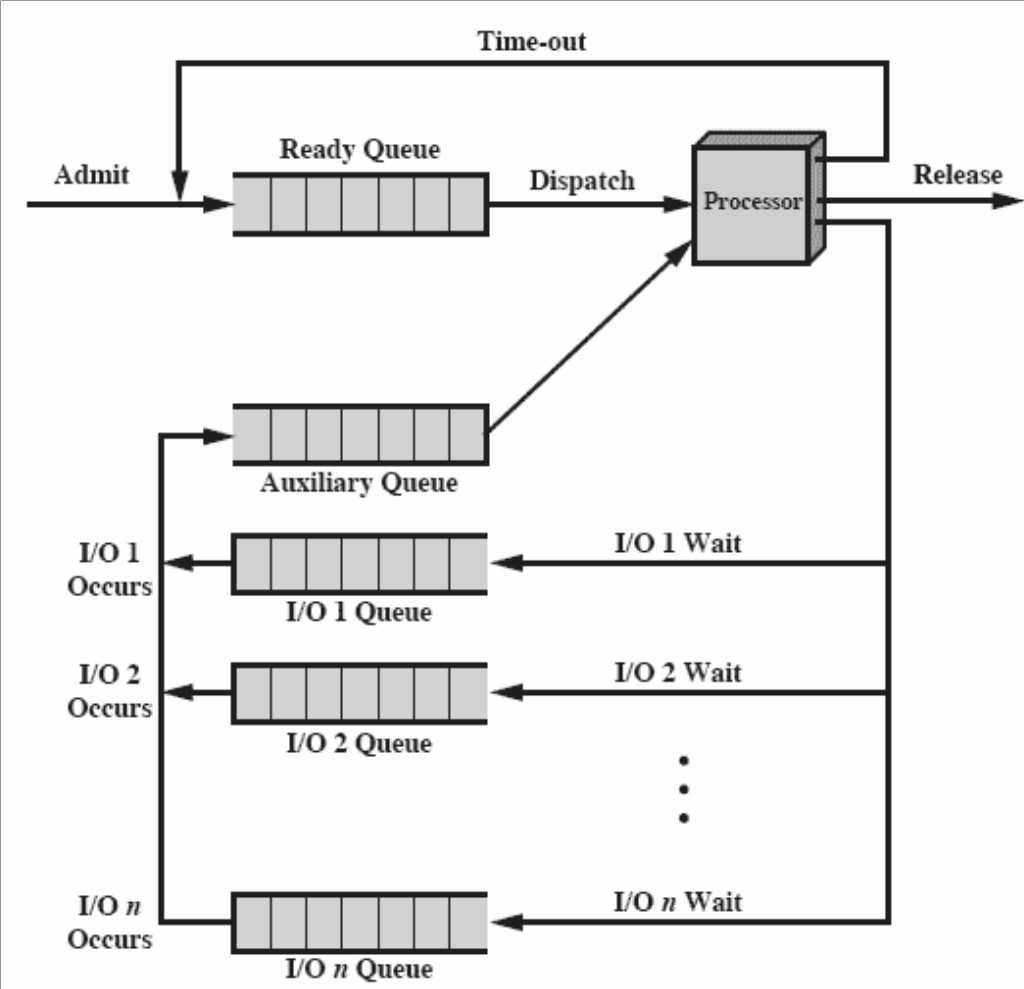
\includegraphics[width=4in]{img/virtualroundrobin.png}
        \caption{Virtual Round Robin voorbeeld}
    \label{fig:Virtual Round Robin voorbeeld}
\end{figure}

\textbf{Shortest Process Next}

Dit is een niet-preëmptieve strategie. Het proces met de kleinste verwachte uitvoeringstijd wordt als volgende geselecteerd. Het kortste proces springt dan voorbij langere processen naar het begin van de wachtrij.

\begin{figure}[htp]
    \centering
            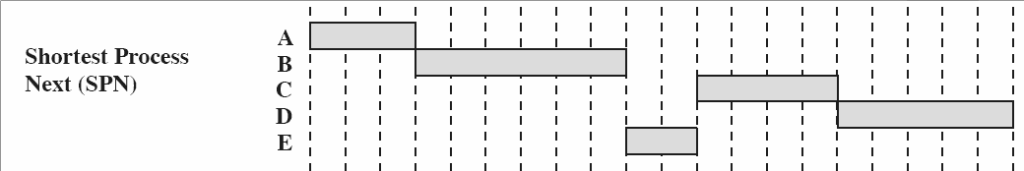
\includegraphics[width=4in]{img/spn.png}
        \caption{Shortest Process Next voorbeeld}
    \label{fig:Shortest Process Next voorbeeld}
\end{figure}

Stel dat de geschatte tijd voor een proces niet juist is, dan kan het besturingssysteem het proces onderbreken. De mogelijkheid bestaat dat langere processen aan starvation lijden.

\textbf{Shortest Remaining Time}

Preëmptieve versie van shortest process next strategie. Moet ook de proces tijd schatten en het kortste uitkiezen.

\begin{figure}[htp]
    \centering
            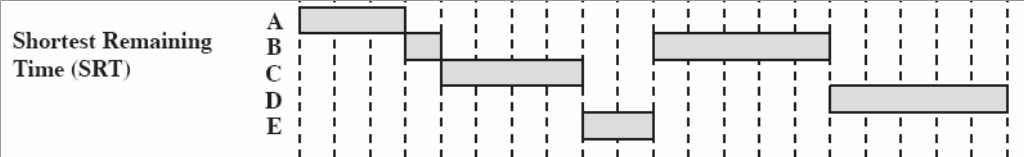
\includegraphics[width=4in]{img/srt.png}
        \caption{Shortest Remaining Time voorbeeld}
    \label{fig:Shortest Remaining Time voorbeeld}
\end{figure}

\textbf{Highest Response Ratio Next}

Deze strategie kiest het volgende proces met de beste ratio.
Ratio = (tijd gespendeerd wachten + verwachte service tijd) / verwachte service tijd

\begin{comment}

\begin{figure}[htp]
    \centering
            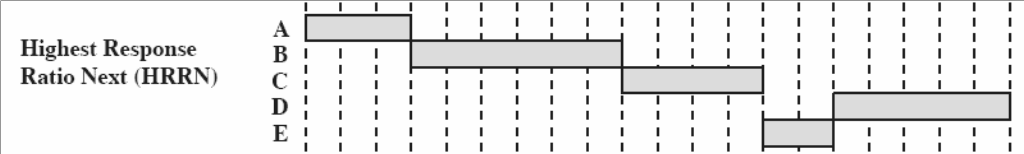
\includegraphics[width=4in]{img/hrrn.png}
        \caption{Highest Response Ratio Next voorbeeld}
    \label{fig:Highest Response Ratio Next voorbeeld}
\end{figure}

\end{comment}


%To prevent floating at all we must not use the figure environment. The caption package gives a way to get all the other features. It provides the command \captionof that takes a counter (figure or table) as argument and of course the caption text, for example:
\begin{center}
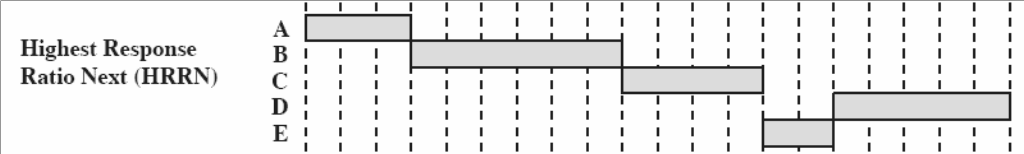
\includegraphics[width=4in]{img/hrrn.png}
\captionof{figure}{Highest Response Ratio Next voorbeeld}\label{Highest Response Ratio Next voorbeeld}%
\end{center}

\textbf{Feedback Scheduling}

Een nieuw proces komt binnen en krijgt een hoge prioriteit. Elke keer dat hij uitvoeringstijd kreeg, gaat zijn prioriteit een niveau omlaag en komt hij in een wachtrij met een lagere prioriteit.

\begin{comment}

\begin{figure}[htp]
    \centering
            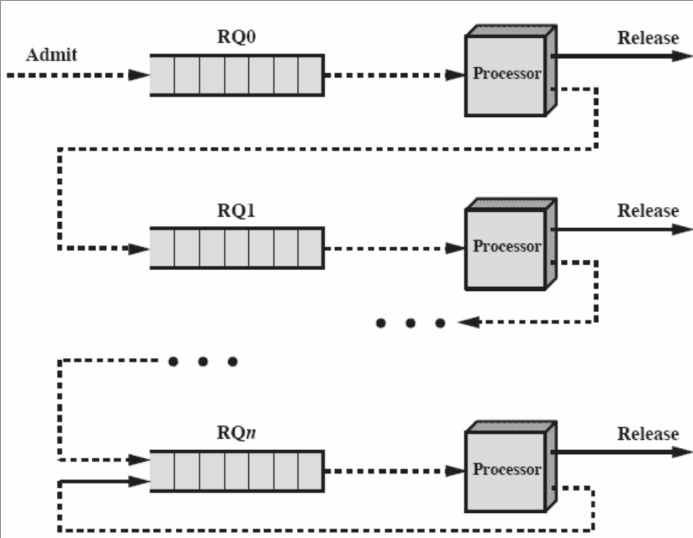
\includegraphics[width=4in]{img/feedbackscheduling.png}
        \caption{Feedback Scheduling voorbeeld}
    \label{fig:Feedback Scheduling voorbeeld}
\end{figure}

\end{comment}



Problemen zijn dat er niet geweten is hoeveel tijd er nog nodig is om het programma uit te voeren en dat grote processen aan starvation kunnen lijden moesten er continu nieuwe processen binnenkomen.

Oplossing hierbij kan zijn om processen de mogelijkheid te geven om zichzelf te promoveren naar een wachtrij met een hogere prioriteit nadat het een tijd niet aan bod zou mogen gekomen zijn.




\textbf{Feedback Performance}

Variaties bestaan, dit is preëmptief op klokinterrupt. Het is vergelijkbaar met Round Robin. Het kan tot starvation leiden!

\begin{figure}[htp]
    \centering
            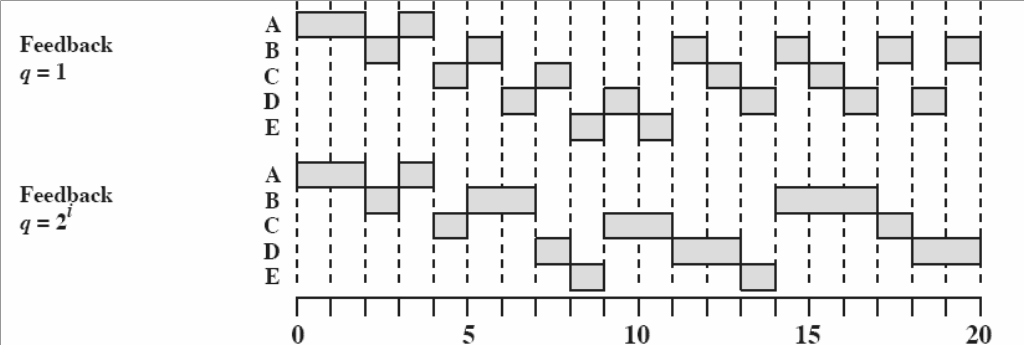
\includegraphics[width=4in]{img/feedbackperformance.png}
        \caption{Feedback Performance voorbeeld}
    \label{fig:Feedback Performance voorbeeld}
\end{figure}












